\documentclass[11pt]{article}
\usepackage[brazilian]{babel}
\usepackage[utf8]{inputenc} %acentuação da língua portuguesa
\usepackage[T1]{fontenc} 
\usepackage{wrapfig} %figura ao lado do texto
\usepackage{graphicx} %pacote de figuras

\usepackage{amsfonts} %pacote com \mathbb{}

\usepackage[pdftex]{hyperref} %links da internet

\usepackage{fancyhdr} 

\usepackage{hyphenat} %retirar hefenação

\tolerance=1 %retirar hefenação

\emergencystretch=\maxdimen %retirar hefenação

\hyphenpenalty=10000 %retirar hefenação

\hbadness=10000 %retirar hefenação

\hyphenchar\font=-1 %retirar hefenação

\sloppy %retirar hefenação

\usepackage{textcomp}

\usepackage[a4paper,left=2cm,right=2cm,top=2.5cm,bottom=2cm]{geometry}

\setlength{\parindent}{0pt} %Parágrafo sem identação]

\begin{document}
	
	\pagestyle{fancy}
	\renewcommand{\headrulewidth}{0pt}
	\renewcommand{\footrulewidth}{2.1pt}
	\fancyfoot[L]{\small Diego Silveira Costa Nascimento}
	\fancyfoot[R]{\small diego.nascimento@ifrn.edu.br}
	
	\begin{minipage}[c][1.5cm][c]{3cm}
		\begin{flushleft}
			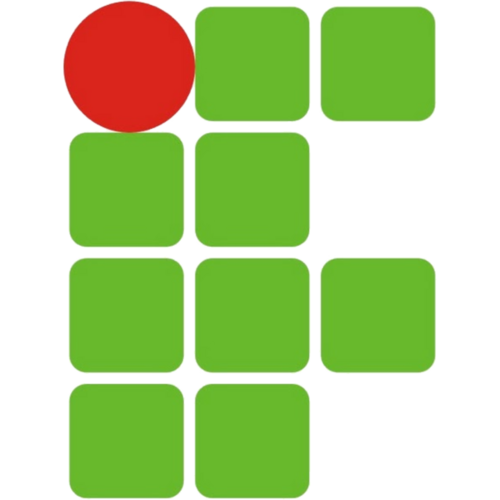
\includegraphics[scale=0.25]{IFRN}
		\end{flushleft}
	\end{minipage}		
	\begin{minipage}[c][1.5cm][c]{10.8cm}
		\begin{center}
			\resizebox{!}{0.3cm}{\textbf{Informática}}\par
			\resizebox{!}{0.2cm}{\textbf{Instituto Federal de Educação, Ciência e Tecnologia do Rio Grande do Norte}}\par
			\resizebox{!}{0.2cm}{\today}
		\end{center}
	\end{minipage}
	
	\begin{center}
		Exercícios
	\end{center}
	
	\section{Introdu\c cão}
	
	\begin{enumerate}
		\item Quais opera\c cões são possíveis de ser calculadas com o ábaco, e como é utilizado?
		\item Quais opera\c cões são possíveis de ser calculadas com o Bastões de Napier, e como é utilizado?
		\item Qual a precursora das calculadoras mecânicas, e qual opera\c cão é realizava?
		\item Quais os tipos de operações realizadas pela calculadora mecânica Leibnitz?
		\item Qual o componente utilizado no tear mecânico, que posteriormente foi utilizado para projetar máquinas de calcular?
		\item Quem é considerado o Pai da Computa\c cão, e por quê?
		\item Quais tipos de operações são realizadas pela Máquina Diferencial de Babbage?
		\item Quais as principais evoluções da Máquina Analítica de Babbage?
		\item Para que foi projetada a máquina de Tabula de Hollerith, e por quê?
		\item Para que serve um computômetro?
		\item Qual o primeiro computador a utilizar cálculos baseado em aritmética binária, e por quem foi desenvolvido?
		\item Para que foi projetado o Colossus?
		\item Qual as gera\c cões dos computadores? Cite suas características.
		\item Qual o primeiro computador eletrônico digital de propósito geral, e suas características?
		\item Qual o primeiro computador comercial entregue a um cliente?
		\item O que é um mainframe?
		\item Qual o primeiro computador desenvolvido para fins pessoal, que trazia recursos como monitor e teclado?
		\item Qual o primeiro computador comercial a possuir interface gráfica e uso do mouse?
	\end{enumerate}
	
	\newpage
	\section{Ergonomia}
	\begin{enumerate}
		\item Qual os objetivos em se preocupar com aspectos de ergonomia com o uso dos computadores?
		\item Descreva quais cuidados devemos ter ao utilizar o computador de forma ergonômica para: visão; punhos e bra\c cos; costa; e os pés.
		\item Pesquise os principais problemas decorrente do mal sudo do computador.
	\end{enumerate}
	
	\newpage
	\section{Hardware}
	
	\begin{enumerate}
		\item O que é hardware?
		\item O que é um placa-mãe e sua finalidade?
		\item O que é um processador, em quais partes é organizado, e qual a fun\c cão de cada uma delas?
		\item Quais o tipos de memória, e para que serve cada uma delas?
		\item Quais o tipos de periféricos? Cite exemplos de cada um deles.
		\item Quais os tipos de impressoras? Cite quais são as vantagens e desvantagens de cada uma delas.
	\end{enumerate}

	\newpage
	\section{Software}
	
	\begin{enumerate}
		\item O que é software?
		\item O que é software de sistema? Cite exemplos.
		\item Quais as principais tarefas do software de sistema?
		\item O que é software de aplicativo?
		\item Quais os tipos de softwares aplicativos?
		\item O que é um software editor de texto, quais suas características? Cite exemplos.
		\item O que é um software editor de planilha eletrônica, quais suas características? Cite exemplos.
		\item O que é um software de produção, quais suas características? Cite exemplos.
		\item O que é um software de gerenciamento de informação pessoal, quais suas características? Cite exemplos.
		\item O que é um software de comunicação, quais suas características? Cite exemplos.
	\end{enumerate}

	\newpage
	\section{Sistema Operacional}
	
		\begin{enumerate}
			\item O que é um sistema operacional?
			\item Quais as características de um sistema operacional?
			\item Quais as tarefas básicas de um sistema operacional?
			\item Cite cinco sistemas operacionais.
			\item	Abra o aplicativa da calculadora.
			\item Altere a configura\c cão da calculadora para científica.
			\item Abra o diretório de documentos, e em seguida crie a estrutura de pastas a seguir:\\
IFRN\\
$+$ Informática\\
-- Exercícios\\
-- Trabalhos\\
$+$ Matemática\\
-- Exercícios\\
-- Trabalhos\\
$+$ Outros\\
-- Vídeos\\
-- Apresentações\\
-- Documentos\\
	\end{enumerate}
		
	\newpage
	\section{Internet}
	
	\begin{enumerate}
		\item O que é internet?
		\item Quais os tipos de conexões que permitem o acesso à internet? Para cada uma delas, cite as vantagens e desvantagens.
		\item O que é uma página na internet?
		\item O que é uma URL e em quantas partes são divididas?
		\item O que é um navegador? Cite os mais conhecidos.
		\item Abra um navegador da sua preferência e acesse a página do IFRN no endere\c co \url{www.ifrn.edu.br}.
		\item Ainda no navegador, abra uma nova aba, e acesso a página do SUAP no endere\c co \url{suap.ifrn.edu.br}.
		\item Marque a página do SUAP como sua favorita.
		\item Abra um janela anônima no seu navegador, e acesse o e-mail da sua conta pessoal.
		\item Quais os principais servi\c cos de e-mails disponíveis no mercado?
		\item Escreva um e-mail para um de seus colegas da turma, contendo assunto, conteúdo e anexo de um arquivo qualquer.
		\item Escreva um e-mail para dois ou mais colegas da sua turma, contendo assunto e conteúdo.
		\item Escreva um e-mail para dois ou mais colegas da sua turma, contendo assunto e conteúdo, sendo que pelo menos um dos destinatários deverá receber a mensagem como cópia (Cc).
		\item Escreva um e-mail para dois ou mais colegas da sua turma, contendo assunto e conteúdo, sendo que pelo menos um dos destinatários deverá receber a mensagem como cópia oculta (Cco).
		\item Quais os principais servi\c cos de armazenamento em nuvem disponíveis no mercado?
		\item Acesse o seu servi\c co de armazenamento em nuvem, e em seguida crie a estrutura de pastas a seguir:\\
IFRN\\
$+$ Informática\\
-- Exercícios\\
-- Trabalhos\\
$+$ Matemática\\
-- Exercícios\\
-- Trabalhos\\
$+$ Outros\\
-- Vídeos\\
-- Apresentações\\
-- Documentos\\
		\item Fa\c ca o registro dos dias de aula de informática na sua agenda.
		\item Liste as tarefas que você precisa fazer na semana, no gerenciador de tarefas.
		\item Fa\c ca as anota\c cões dos principais conteúdos da disciplina, no gerenciador de notas.
	\end{enumerate}
	
	\newpage
	\section{Editor de Texto}
	
	\begin{enumerate}
		\item Criar um documento de texto contendo contendo seus dados pessoais nome e endere\c co.
		\item Renomeio o arquivo da questão 1 para Exercício 1.
		\item Abrir o arquivo criado na questão 1, e em seguida gerar um versão do documento no formato de leitura PDF.
		\item Cria um documento que contenha uma tabelas com os horários de aula do seu curso.
		\item Criar um documento que contenha várias imagens de capitais do mundo.
		\item Criar uma lista de assinatura de presença com campos para nome, data e assinatura.
		\item Criar uma capa de trabalho que contenha os dados a seguir: nome da instituição de ensino, título do trabalho, nome do aluno, local e data.
		\item Usando um modelo existente do editor de texto, elabore seu currículo profissional.
	\end{enumerate}

	\newpage
	\section{Editor de Apresenta\c cão}

	\begin{enumerate}
		\item Criar uma apresentação no editor de apresenta\c cão.
		\item O conteúdo um conteúdo da sua preferência.
		\item Criar no mínio 5 slides com diferentes layouts.
		\item Escolha um tema padrão para todos os slides.
		\item Aplicar efeitos de transição em todos os slides.
		\item Aplicar animações.
	\end{enumerate}

	\newpage
	\section{Editor de Planilha}

	\begin{enumerate}
		\item Criar uma planilha em branco, em seguida renome-a com o nome Controle de Notas.
		\item Aplicar a formatação nas colunas 1º Bimestre, 2º Bimestre, 3º Bimestre e 4º Bimestre, para exibir as notas no formato de número real, com uma casa decimal separada por vírgula.
		\item Criar uma fórmula (não usar função já definida), na coluna média, para o cálculo da média das notas de todos os bimestres.
		\item Usar a função “se” para informar a situação do aluno de forma automática, informando se o mesmo está “Aprovado” ou “Reprovado”, assumindo que o aluno está aprovado se sua média nos quatro bimestre for maior ou igual a 7,0, ou reprovado, caso contrário.
		\item Criar um gráfico em barra, para uma análise comparativa, das notas de todas as disciplinas nos quatro bimestres.
	\end{enumerate}

\end{document}